
% \documentclass[fleqn,10pt]{wlscirep}
% fleqn : left alignment of equation

\documentclass[10pt]{wlscirep}
\usepackage[utf8]{inputenc}
\usepackage{amsmath}
\usepackage{amsbsy}
\usepackage{xcolor}
\usepackage[T1]{fontenc}
\usepackage{soul} % 여러 라인에 걸친 밑줄을 사용하기 위한 패키지

\DeclareMathOperator*{\argmin}{arg\,min} % Jan Hlavacek

%from here, code for line numbers
\usepackage{lineno}
\linenumbers

\makeatletter
\patchcmd\@maketitle{%
        {%
        \noindent
        \colorbox{color2}{%
            \parbox{\dimexpr\linewidth-2\fboxsep\relax}{%
            \sffamily\small\textbf\\\theabstract
            }%
        }%
        }%
    }{%
        \nolinenumbers{%
        \noindent
        \colorbox{color2}{%
            \parbox{\dimexpr\linewidth-2\fboxsep\relax}{%
            \internallinenumbers \sffamily\small\theabstract
            }%
        }%
        }%
    }
    {\wlog{true}}{\wlog{false}}
    
\makeatother
%end of code for line numbers

\title{Radionuclide Identification for Plastic Scintillation Detectors by Backward Cumulative Channel Sum}
% \linenumbers
\author[1]{Ji-Yong So}
\author[2]{Byoungil Jeon}
\author[1,*]{Myungkook Moon}
\affil[1]{Korea Atomic Energy Research Institute, Neutron Science Division, Daejeon, 34057, Korea}
\affil[2]{Korea Atomic Energy Research Institute, Applied Artificial Intelligence Section, Daejeon, 34057, Korea}

\affil[*]{moonmk@kaeri.re.kr}

% \affil[+]{These authors equally contributed to this work}

\keywords{radiation portal monitor, radionuclide identification}

\begin{abstract}

Plastic scintillation detectors are widely used in radiation monitoring systems because of their high detection efficiency, fast response, and robust operation. However, reliable radionuclide discrimination remains difficult because plastic scintillators exhibit low energy resolution, broad Compton-dominated spectral distributions, and strong sensitivity to background variation in practical measurement environments. 

In this study, we propose a backward cumulative channel sum (BCCS)-based spectral processing framework for improving radionuclide discrimination using large plastic scintillation detectors. The proposed method preserves the intrinsic spectral characteristics of plastic scintillators while reducing statistical fluctuations through cumulative transformation. After BCCS preprocessing, subtraction-based and normalization-based background compensation methods were applied, and the processed spectra were analyzed using a linear spectral unfolding framework.

The method was evaluated using Am-241, Cs-137, and Co-60 under both single-source and mixed-source conditions. The results showed that the BCCS transformation provides a more stable spectral representation than the raw spectrum, enhances radionuclide-dependent spectral contrast, and enables practical decomposition of mixed-source spectra. The subtraction-based method preserved net count-scale information, whereas the normalization-based method provided improved robustness under varying acquisition conditions.

Overall, the proposed BCCS-based framework provides a practical and physically meaningful approach for extracting radionuclide-specific information from low-resolution plastic scintillator spectra under low-count, mixed-source, and background-varying conditions, and is expected to be useful for real-time radiation monitoring and container
inspection applications.

\end{abstract} 

\begin{document}

\flushbottom
\maketitle

\thispagestyle{empty}


\section*{Introduction}

Plastic scintillation detectors are widely used in radiation portal monitors (RPMs) and other
field-deployable radiation monitoring systems because of their high detection efficiency, fast response, and robust operation\cite{Sicilliano2005Comparision, Bertrand2014Current,Ely2006TheUse,Hevener2013EWindow}. However, reliable radionuclide identification using plastic scintillators remains challenging because of their inherently poor energy resolution and broad spectral distributions dominated by Compton scattering\cite{Hevener2013EWindow, Lee2020Radioisotope, Paff2017Spectral,Runkle2006Analysis}. 

This difficulty becomes more significant in practical RPM environments. During container inspection, the container itself and the cargo inside it can partially attenuate radiation and alter the measured background spectrum. As a result, background intensity and spectral shape may vary depending on the inspected object, making radionuclide discrimination based only on gross counts unreliable \cite{Lee2020Radioisotope, Paff2017Spectral,Runkle2006Analysis,Kim2019InvMat}. Under such conditions, more effective use of spectral shape information is required.

Under identical background conditions, the spectral response of a given radionuclide preserves its overall shape while its amplitude scales with source intensity. Although discrete counting statistics introduce small fluctuations, the characteristic spectral pattern remains stable. This property provides the basis for constructing radionuclide-specific reference spectra and for interpreting mixed-source measurements as linear combinations of these reference patterns.

Several approaches have been proposed to improve radionuclide identification in low-resolution detectors, including spectral windowing, statistical feature extraction, unfolding-based methods, and machine-learning-based classification [7–11,13–16]. However, their practical applicability may be limited in real RPM environments, where a container truck passes the detector within a short time and a localized radioactive source contributes significantly to the measured spectrum only during a brief interval when it is close to the detector. Under such conditions, the measured signal is often affected by limited counting statistics, variable background, and mixed-source characteristics.

In this study, we propose a backward cumulative channel sum (BCCS)-based spectral processing method for plastic scintillation detectors. The proposed method uses the full spectral information while reducing statistical fluctuations through cumulative transformation, thereby preserving the global spectral shape and enhancing subtle differences between radionuclides. Once radionuclide-specific reference spectra are transformed into the BCCS domain, mixtures of multiple radionuclides can be analyzed using a least-squares-based decomposition framework to estimate their relative
contributions.

% To evaluate the characteristics of the proposed method, three representative radionuclides—Am-241, Cs-137, and Co-60—were selected in this study. These radionuclides have relatively long half-lives and distinct energy distributions, making them suitable for assessing the performance of the BCCS-based approach under both single-source and mixed-source conditions.

\color{red}To evaluate the proposed BCCS-based approach, three representative radionuclides—Am-241, Cs-137, and Co-60—were selected as test cases. These radionuclides have relatively long half-lives and exhibit distinct spectral characteristics in plastic scintillation detectors and thus provide a practical basis for assessing the method under both single-source and mixed-source conditions.\normalcolor

\section*{Methods}
\subsection*{Experimental Setup}

All measurements were performed using the same plastic scintillation detector system under identical detector geometry conditions. The detector consisted of a plastic scintillator
with dimensions of 30 cm $\times$ 180 cm $\times$ 5 cm, coupled to a photomultiplier tube (PMT). The
detector size and measurement configuration were kept unchanged throughout the experiments in order to ensure consistent comparison among single-source, mixed-source, and background measurements.

Background measurements were acquired in the absence of any radioactive source. The background count rate depended slightly on the lower level discriminator (LLD) setting. Under the measurement condition used in this study, where the LLD was set to include the energy region relevant to Am-241 detection, the background count rate was approximately 10,000 cps per detector. This background condition was used as the reference for both subtraction-based and normalization-based spectral processing.

% Three representative radionuclides, Am-241, Cs-137, and Co-60, were selected for evaluation of the proposed method. These radionuclides were chosen because they have relatively long half-lives and distinct representative energy regions, allowing systematic comparison of their spectral characteristics. In addition to single-source measurements, mixed-source conditions were also prepared to evaluate decomposition performance.
\color{red}
The experimental evaluation was performed using Am-241, Cs-137, and Co-60. Single-source measurements were used to construct radionuclide-specific reference spectra, and mixed-source configurations were additionally prepared to evaluate decomposition performance.
\normalcolor
\subsection*{Spectral Channel Configuration}

In scintillation detector systems, spectral data are commonly acquired using 256, 512, or 1024 channels, whereas high-resolution semiconductor detectors such as HPGe often use much finer channel configurations, such as 4k or 8k channels. However, for plastic scintillation detectors, increasing the number of channels does not necessarily improve radionuclide discrimination because of the intrinsically low energy resolution of the detector response.

In this study, the spectral data were analyzed using 256 channels. The reason for this choice is that increasing the number of channels reduces the counts per channel and degrades counting statistics, while providing little additional discriminative information for plastic scintillator spectra. Therefore, the use of 256 channels provides a practical balance between spectral representation and statistical reliability for plastic scintillator-based measurements. This choice is particularly appropriate for plastic scintillation detectors, in which statistical
fluctuations are more influential than fine spectral resolution.


\subsection*{Spectral Preprocessing: Backward Cumulative Channel Sum (BCCS)}
\color{red}
The backward cumulative channel sum (BCCS) is defined as a cumulative transformation of the pulse-height spectrum. Let $\mathbf{C} = [C_1,\,C_2,\ldots,\,C_N]$ denote the raw pulse-height spectrum, where $C_i$ is the count in channel $i$. The BCCS spectrum is given by

\begin{equation}
B_i = \sum_{j=i}^N C_j. \label{eq:BCCS}
\end{equation}

This transformation produces a monotonically decreasing representation of the spectrum, reducing statistical fluctuations while preserving the global spectral shape. Because plastic scintillator spectra are dominated by broad Compton-related distributions rather than sharp photopeaks, preservation of the overall spectral shape is more important than retaining fine channel-by-channel variations.


During method development, both forward and backward cumulative summation schemes were examined. The forward cumulative sum is defined as

$$
F_i = \sum_{j=1}^i C_j. \label{eq_FCCS}
$$

In the forward cumulative representation, the cumulative values are constructed from the lowest channels upward. Because the spectral features relevant for radionuclide discrimination in plastic scintillators are primarily located in the low- to medium-channel region, the forward scheme provides limited noise suppression in these critical channels. As a result, statistical fluctuations in the most informative part of the spectrum remain largely unmitigated.
In contrast, the backward cumulative representation integrates counts from each channel toward the high-channel end of the spectrum. This leads to substantial averaging even in the low- and medium-channel region, where most of the physically meaningful spectral differences reside. Consequently, the backward scheme more effectively reduces statistical fluctuations in the most relevant part of the spectrum while preserving the global spectral trend.
For these reasons, the backward cumulative channel sum (BCCS) was adopted in this study as the primary spectral transformation method.
\normalcolor

For each measurement condition, repeated acquisitions were performed more than 10 times under identical experimental settings. Because the run-to-run variation in spectral shape and in the resulting BCCS trend was negligible, a single representative spectrum is presented in the figures for clarity.

% Unlike the conventional forward cumulative spectrum that sums from the first channel upward, the BCCS accumulates counts from channel 
% $i$ to the end of the spectrum. This produces a smooth, monotonically decreasing cumulative profile that suppresses statistical fluctuations in the high-channel region while preserving the global spectral structure. Because this transform enhances separability under low-count conditions, it serves as the primary preprocessing step for all subsequent analyses.


\subsection*{Background Compensation Techniques}

After BCCS preprocessing, background compensation was applied to reduce the influence of ambient radiation and system background on the transformed spectra. \color{red}In practical RPM environments, both the intensity and spectral shape of the background may vary depending on container structure, cargo composition, and measurement conditions. Therefore, appropriate background compensation is essential prior to radionuclides spectral decomposition.

Two background compensation techniques were considered in this study. The first was a subtraction-based method, \color{red}efined as 

\begin{equation}
S^X_i =  B^X_i - B_i^{\textrm{bkg}}. \label{eq:DS}
\end{equation}

where $B_i^X$ and $B_i^\text{bkg}$ denotes BCCS spectra of the measured signal and background, respectively. This approach preserves the net count scale of the source contribution and is suitable when absolute signal magnitude is relevant for interpretation, although it may also amplify statistical fluctuations when the count level is low.

The second was a normalization-based method, defined as 

\begin{equation}
R^X_i = \left(\dfrac{B^X_i}{B^{\textrm{bkg}}_i}\right) -1.\label{eq:NB}
\end{equation}

This formulation represents the relative deviation of the measured spectrum from the background. The subtraction of unity ensures that 
$R_i^X = 0$ corresponds to pure background, providing a convenient baseline for comparison. Because the ratio removes the common scaling factor between the measured and background spectra, it is largely independent of acquisition time and overall count scale. This property is particularly useful in real-time inspection systems, where the effective measurement time may vary as a container truck passes the detector.\normalcolor

In both compensation schemes, the spectral data can also be converted into count-rate form by dividing the measured counts by the acquisition time. In this case, the {\color{red}spectral} values are no longer restricted to integers and may take fractional values. However, this does not affect the BCCS procedure, because the cumulative summation can be applied equally to integer and non-integer values. Therefore, the proposed method remains applicable even when the measurement time varies. This property is particularly important in practical RPM environments, where container trucks do not always pass the detector at a constant speed.

Both compensation methods were applied in the BCCS domain, and their performances were compared in terms of spectral contrast, stability, and robustness in subsequent decomposition analysis.

\subsection*{Radionuclide Activity Estimation via Linear Spectral Unfolding}

Following BCCS preprocessing and background compensation, the processed spectra were analyzed using a linear spectral unfolding framework. The basis of this approach is the experimental observation that, under identical background conditions, each radionuclide produces a characteristic spectral pattern whose overall shape remains nearly unchanged while its amplitude scales with source intensity. Although discrete counting statistics introduce small deviations, the underlying spectral shape remains sufficiently stable for reference-based decomposition.

Based on this property, radionuclide-specific reference spectra were constructed in the BCCS domain. A measured spectrum containing one or more radionuclides was then represented as a linear combination of these reference BCCS spectra.

\begin{equation}
S_i^M = \sum_X \alpha_X S_i^X,\label{eq:submethod}
\end{equation}

\noindent where $\alpha_X$ denotes its contribution. Because meaningful spectral features are present only in the lower channels for plastic scintillators under low-count conditions, the unfolding is performed over the restricted channel range. Similary, for the ratio-normalized spectra, we obtain

\begin{equation*}
R_i^M = \sum_X \alpha_X \left(\dfrac{S_i^X}{B_i^{M,\text{bkg}}}\right).
\end{equation*}

If the background distributions of the measured spectrum and reference spectra are comparable, i.e., $B^{M,\text{bkg}}_i \approx B_i^{X,\text{bkg}}$, then

\begin{equation}
R_i^M = \sum_X \alpha_X \left(\dfrac{S_i^X}{B_i^{X,\text{bkg}}}\right) = \sum_X \alpha_X R_i^X.\label{eq:ratiomethod}
\end{equation}

In both cases-direct subtraction (\ref{eq:submethod}) and ratio normalization (\ref{eq:ratiomethod})-the coefficients $\alpha_X$ can be estimated by solving the non-negative least squares (NNLS) problem :

\begin{equation}
\argmin_{\alpha_X \ge 0} \left\| \textbf{I}^{\text{M}} - \sum_{X} \alpha_X \textbf{I}^{X}\right\|^2,\label{eqn:llns}
\end{equation}

where $\bf{I}^M$ and $\bf{I}^{X}$ denote the measured and reference spectra after applying the chosen background compensation method.

This procedure does not aim to determine the absolute activity of each radionuclide in becquerels, because the moving container geometry does not permit direct activity quantification. Instead, the resulting coefficients are interpreted as reference-based indicators of the relative contribution and relative signal level of each radionuclide in the measured detector response. Therefore, the proposed method can be used to identify which radionuclides are present and to assess their relative strength with respect to the corresponding reference conditions.

\section*{Results}

%Up to three levels of \textbf{subheading} are permitted. Subheadings should not be numbered.

\subsection*{Spectral Transformation of Reference Radionuclides Spectra}

Figure \ref{fig:bkgref}(a) shows the raw spectra of background radiation and three reference radionuclides, Am-241, Cs-137, and Co-60, measured using a large-volume plastic scintillation detector. As expected for plastic scintillators, the spectra are dominated by broad Compton continua rather than sharp photopeaks, and most counts are concentrated in the low-channel region. Under these conditions, direct visual discrimination from the raw spectra is limited, especially for weak sources or low net-count situations.

After applying the BCCS transformation yields smooth and monotonically decreasing profiles, as shown in Figure \ref{fig:bkgref}(b). The transformation reduces channel-to-channel statistical fluctuations while preserving the global spectral shape of each radionuclide. Thus, the BCCS representation provides a more stable basis for qualitative comparison and subsequent decomposition analysis. 

Figures \ref{fig:bkgref} (c) and \ref{fig:bkgref} (d) show the background-subtracted and background-normalized BCCS spectra, respectively. The subtraction-based representation preserves the absolute scale of the net source signal, whereas the normalization-based representation enhances relative deviations from background. Both representations improve radionuclide-specific contrast compared with the raw spectra, although in different ways.

It should be noted that the small Am-241 values observed in the high-channel region do not have physical significance. They originate from statistical fluctuations in the measured low-count data and were retained as part of the original experimental dataset without artificial suppression.

\subsection*{Comparison of background compensation methods for mixed-source spectra}

Figure \ref{fig:mixedbccs} presents the BCCS spectra for nine mixed-source configurations obtained using the two background compensation methods. In Fig.\ref{fig:mixedbccs}(a), the subtraction-based BCCS spectra preserve absolute count differences among mixtures, making it possible to compare both spectral shape and relative signal magnitude. This representation is useful when count-scale information needs to be retained for reference-based fitting.

In contrast, Fig. \ref{fig:mixedbccs}(b) shows that background normalization produces a dimensionless representation with improved visual contrast among mixed-source cases. Because the normalized values reflect deviations relative to background, the method is less sensitive to measurement time and overall count-scale variation. This is particularly useful in RPM applications, where effective acquisition time may vary as a truck passes the detector.

The two compensation methods therefore play complementary roles. Subtraction preserves absolute signal information, whereas normalization provides greater flexibility under varying acquisition conditions.


\subsection*{Linear spectral unfolding of mixed-source measurements}

The unfolding results for the mixed-source spectra are shown in Figs. \ref{fig:fi_fitbgsub} and \ref{fig:fi_fitbgrto}. In both cases, the measured BCCS spectrum is well reproduced by the fitted combination of reference radionuclide spectra, indicating that the mixed-source response can be described as a linear combination of radionuclide-specific reference patterns in the BCCS domain.

For the subtraction-based case in Fig. \ref{fig:fi_fitbgsub}, the fitting results show that the net source contribution can be decomposed into Am-241, Cs-137, and Co-60 components with physically meaningful non-negative coefficients. This demonstrates that BCCS preprocessing stabilizes the spectral representation sufficiently for least-squares-based decomposition, despite the low energy resolution of the detector. As in Fig. \ref{fig:bkgref}, the small Am-241 values appearing in the high-channel region are attributable to statistical fluctuations in the original measured data and do not represent physically meaningful spectral structure.

For the normalization-based case in Fig. \ref{fig:fi_fitbgrto}, the decomposition remains stable while providing a representation that is less sensitive to acquisition-time variation. Since BCCS is based on cumulative summation, it can be applied equally to integer-valued spectra and count-rate-based real-valued spectra. Therefore, the method remains applicable even when truck speed and effective counting time vary.

The unfolding was performed over the low-channel region, where the meaningful source information is concentrated for plastic scintillators. This fitting range reduces the influence of high-channel statistical noise while preserving the spectral shape information needed for radionuclide discrimination.


\subsection*{Relative signal level as a function of measurement condition}

Figure \ref{fig:fi_fitcontrib} summarizes the estimated coefficients as a function of source-to-detector distance. As the distance increases, the inferred signal level of the corresponding radionuclide decreases monotonically, which is consistent with geometric attenuation and reduced net counts. At sufficiently large distance, the inferred coefficient approaches the background- derived level, beyond which reliable discrimination becomes difficult.

Importantly, the coefficients obtained in this work should not be interpreted as absolute activities in becquerels. Instead, they represent reference-based relative signal levels, indicating which radionuclides contribute to the measured response and how strong each contribution is relative to the corresponding reference condition.

Overall, the results show that the proposed workflow—BCCS preprocessing, background compensation, and linear spectral unfolding—provides a practical means of extracting radionuclide-specific information from low-resolution plastic scintillator spectra under low-count and mixed-source conditions.

\section*{Discussion}

The effectiveness of the proposed BCCS framework is closely related to the intrinsic response characteristics of plastic scintillation detectors. Because these detectors produce broad Compton-dominated spectral distributions rather than sharp photopeaks, preserving the overall spectral tendency is more important than retaining highly fluctuating channel-by-channel detail. In this context, the BCCS transformation is effective because it preserves the intrinsic spectral shape of the detector response while reducing statistical instability. Thus, the method should be understood not simply as a smoothing procedure, but as a spectral representation strategy tailored to the physical characteristics of plastic scintillators.

Another important advantage of the proposed method is that it makes use of spectral shape information rather than relying only on gross count variation. In practical RPM measurements, the container itself and the cargo inside it can modify both the background level and the measured spectral shape. Under such conditions, radionuclide discrimination based only on total count rate is often insufficient. The BCCS representation provides a more stable way to compare spectra and to identify source-dependent deviations from background, even when the raw spectra appear ambiguous. 

The comparison between subtraction-based and normalization-based compensation also clarifies the practical utility of the framework. Subtraction is useful when preservation of net count-scale information is important, whereas normalization provides a more flexible representation under varying acquisition conditions. Since both methods can be expressed on a count-rate basis, the channel values do not need to remain integers, and this does not affect the BCCS operation. This is particularly relevant for RPM applications, where the speed of a container truck is not strictly constant and the effective measurement time may vary from one measurement to another.

In the present study, the subtraction-based and normalization-based approaches did not produce a substantial difference in radionuclide discrimination performance. Rather than representing competing methods, they should be regarded as complementary background compensation strategies: the subtraction-based method preserves the net signal scale for reference-based interpretation, whereas the normalization-based method provides a more intuitive indication of how much the measured spectrum increases relative to the contemporaneous background. In addition, repeated measurements under identical conditions showed negligible variation in spectral shape and BCCS behavior, supporting the reproducibility of the observed trends.

The present study also supports the interpretation that mixed-source spectra can be described through reference-based amplitude scaling. Under comparable background conditions, each radionuclide preserves a characteristic spectral pattern, while its signal magnitude changes according to source strength. Accordingly, the unfolding coefficients should not be interpreted as absolute activities in becquerels, because direct activity quantification is not feasible for a moving container geometry. Instead, the coefficients are more appropriately interpreted as reference-based indicators of relative signal level and relative contribution. In practical terms, this means that the proposed method can identify which radionuclides are present and assess their relative strength with respect to the corresponding reference conditions.

The present experimental validation was performed using three radionuclides, Am-241, Cs- 137, and Co-60, because these were the representative sources available in the laboratory. However, the proposed framework is not restricted to these three radionuclides. If additional radionuclide-specific reference spectra are obtained, the same BCCS-based processing and decomposition procedure can be extended to a larger set of radionuclides. In this sense, the current study should be regarded as a proof-of-concept validation using a limited but representative group of sources rather than as a restriction of the method itself.

A related observation is that K-40 was also found to be distinguishable in practice, although it was not included in the formal figure-based evaluation of the present study. Despite partial similarity in energy range to Co-60 in low-resolution plastic scintillator spectra, the BCCS representation preserved sufficient shape difference for practical separation. This suggests that the proposed framework may remain useful even for radionuclides with partially overlapping spectral characteristics, although formal validation for K-40 was outside the scope of the present manuscript.

Another practical consideration is the potential variation of plastic scintillator spectra due to environmental factors such as temperature. Temperature-dependent gain drift may slightly modify the measured spectral shape, but the overall spectral tendency is generally preserved. In the present framework, this effect can be mitigated by continuously updating the background spectrum under current environmental conditions. Because both subtraction-based and normalization-based processing rely on comparison with the most recent background measurement, slow variations in detector response can be effectively compensated. Furthermore, the BCCS transformation is inherently less sensitive to local fluctuations and small spectral shifts because it emphasizes global spectral behavior through cumulative summation. From a practical RPM perspective, this is sufficient, since the primary objective is reliable detection of artificial radionuclides rather than precise spectroscopic reconstruction.

Overall, the proposed framework provides a practical and physically well-motivated way to extract radionuclide-specific information from low-resolution plastic scintillator spectra under low-count, mixed-source, and background-varying conditions. Its main strength lies in preserving source-dependent spectral tendencies while reducing statistical instability, thereby enabling stable reference-based decomposition without requiring high-resolution detector hardware or data-intensive learning procedures.

\section*{Conclusion}

In this study, a backward cumulative channel sum (BCCS)-based spectral processing framework was proposed for improving radionuclide discrimination using large plastic scintillation detectors in practical RPM-like environments. The method was designed to preserve the intrinsic spectral characteristics of plastic scintillators while reducing statistical fluctuations, thereby providing a more stable basis for spectral comparison and decomposition.

The results showed that the BCCS transformation enhances radionuclide-dependent spectral contrast by preserving the global spectral shape of the detector response while suppressing local statistical noise. In combination with background compensation and linear spectral unfolding, the proposed framework enables effective analysis of mixed-source spectra under low-count and varying background conditions. Subtraction preserves net count-scale information, whereas normalization provides an important practical advantage when the effective measurement time changes.

The coefficients obtained from the unfolding procedure should not be interpreted as absolute radionuclide activities, but rather as reference-based indicators of relative signal level and relative contribution. This interpretation is more appropriate for practical container inspection systems, where the moving geometry does not permit direct activity quantification but still requires reliable identification of artificial radionuclides and assessment of their relative strength. 

Although the present study formally evaluated three representative radionuclides, the proposed framework is not limited to this set and can be extended whenever additional reference spectra are available. The method therefore provides a practical and physically meaningful approach for extracting radionuclide-specific information from low-resolution plastic scintillator spectra, and it is expected to be useful for real-time radiation monitoring and container inspection applications.

\section*{Acknowledgements}

This research was supported by the Ministry of Oceans and Fisheries, Korea, through the Korea Institute of Marine Science \& Technology Promotion (KIMST) under Project No. 20200611. The authors acknowledge the use of ChatGPT (OpenAI) for language refinement and editorial assistance during the preparation of this manuscript. All scientific content, interpretations, and conclusions presented herein were solely developed and validated by the authors.

\section*{Author contributions statement}
M. Moon conceived the study and performed the experiments. J. So developed the analysis software and performed signal processing. B. Jeon synthesized the test datasets and supported evaluation. All authors contributed to writing and reviewing the manuscript.

\bibliography{./biblio}

\section*{Additional information}

% To include, in this order: \textbf{Accession codes} (where applicable); \textbf{Competing interests} (mandatory statement). 

% The corresponding author is responsible for submitting a \href{http://www.nature.com/srep/policies/index.html#competing}{competing interests statement} on behalf of all authors of the paper. This statement must be included in the submitted article file.


\begin{figure}[ht]
\centering
% 
\includegraphics[width=\linewidth]{figure/fig01_bkgref.pdf}
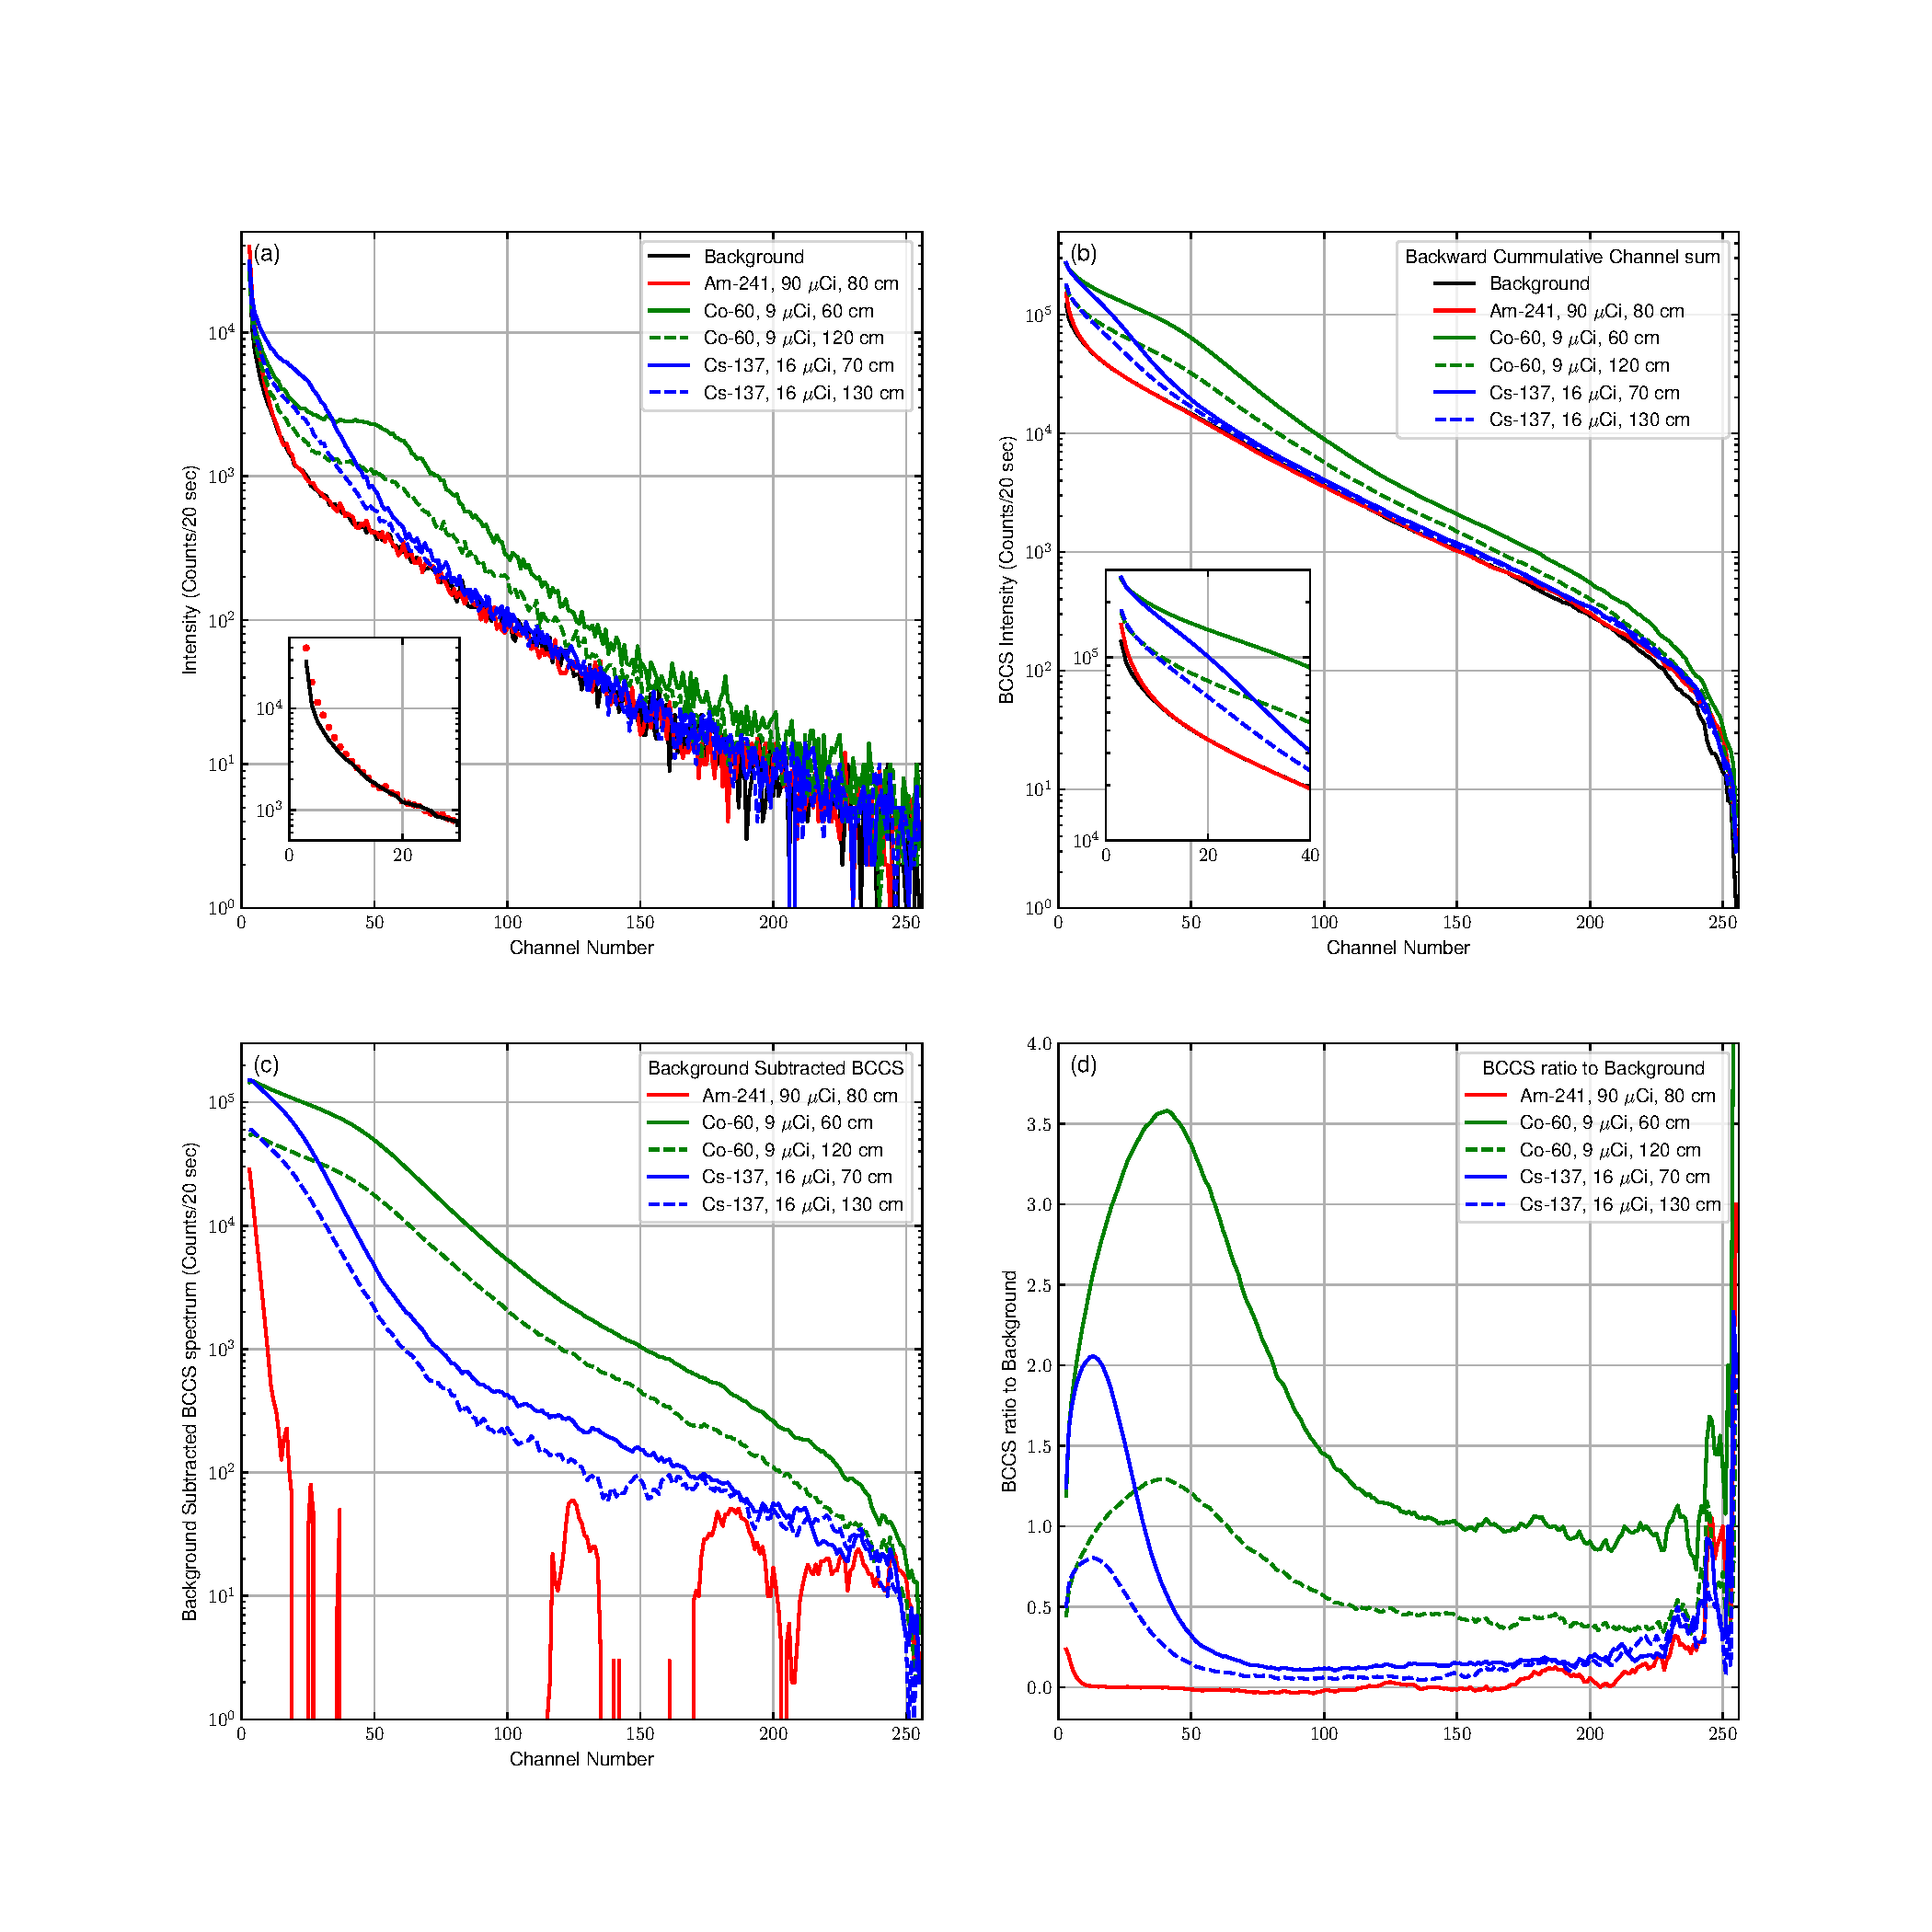
\includegraphics[width=\linewidth]{newfigures/figure1.pdf}
\caption{Spectral comparison of background and reference radionuclides before and after BCCS processing.
(a) Raw spectra of background, Am-241, Cs-137, and Co-60 measured using the plastic scintillation detector.
(b) Corresponding BCCS-transformed spectra.
(c) Background-subtracted BCCS spectra.
(d) Background-normalized BCCS spectra.
The BCCS transformation produces smooth, monotonically decreasing curves while preserving the global spectral characteristics of each radionuclide. The small Am-241 values observed in the high-channel region originate from statistical fluctuations in the measured data and do not represent physically meaningful spectral features.}

\label{fig:bkgref}
\end{figure}

\newpage 

\begin{figure}[ht]
\centering
% 
\includegraphics[width=\linewidth]{figure/fig04_CSBS.pdf}
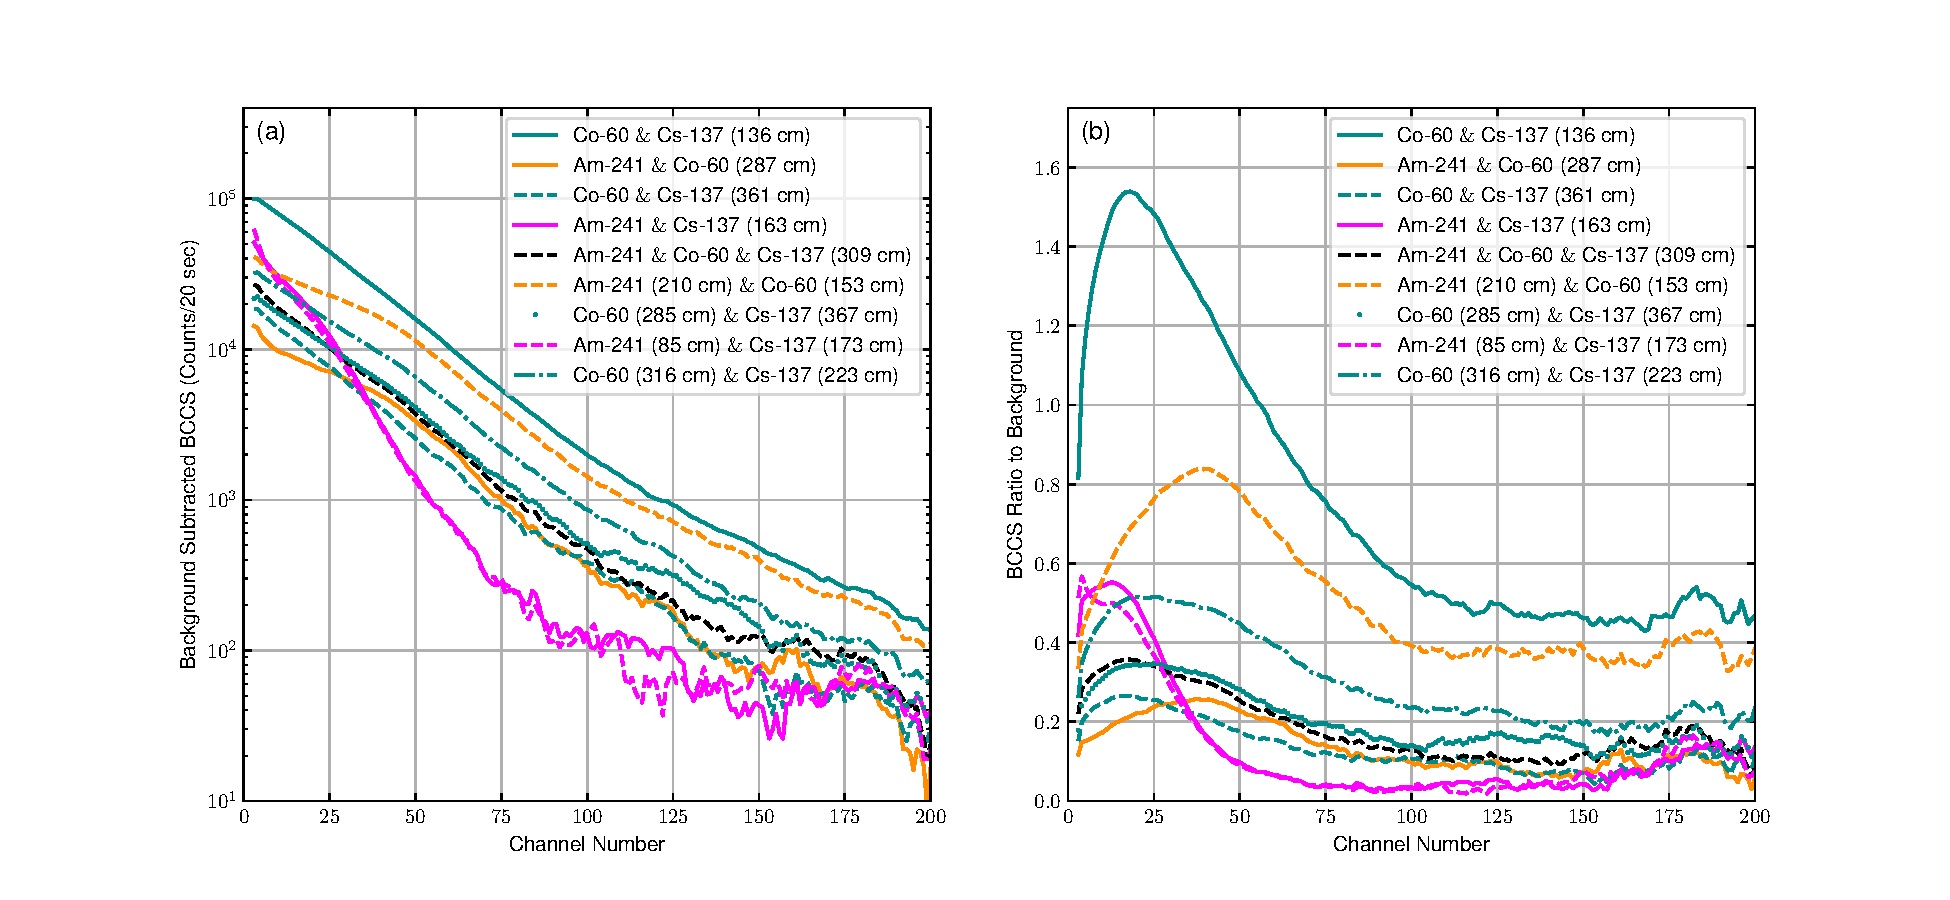
\includegraphics[width=\linewidth]{newfigures/figure2.pdf}
\caption{Comparison of BCCS spectra for mixed-source configurations using different background compensation methods.
(a) Background-subtracted BCCS spectra.
(b) Background-normalized BCCS spectra.
The subtraction-based representation preserves absolute count-scale differences among mixed-source conditions, whereas the normalization-based representation enhances relative deviations from background and provides improved robustness under varying acquisition conditions.}
\label{fig:mixedbccs}
\end{figure}

\newpage


\begin{figure}[ht]
\centering

\includegraphics[width=\linewidth]{newfigures/fit_BGSub.pdf}
\caption{Linear spectral unfolding results for mixed-source spectra using subtraction-based BCCS processing. 
The measured BCCS spectrum (solid line) is fitted by a linear combination of reference radionuclide spectra (dashed lines). The results demonstrate that the mixed-source spectrum can be decomposed into Am-241, Cs-137, and Co-60 components with non-negative coefficients. Minor Am-241 components observed in the high-channel region are attributable to statistical fluctuations and do not represent physically meaningful spectral structure.}
\label{fig:fi_fitbgsub}
\end{figure}

\begin{figure}[ht]
\centering

\includegraphics[width=\linewidth]{newfigures/fit_BGRto.pdf}
\caption{Linear spectral unfolding results for mixed-source spectra using normalization-based BCCS processing.
The measured spectrum is represented in normalized BCCS form and fitted using reference spectra. The normalization-based representation provides stable decomposition while reducing sensitivity to acquisition-time variation. This approach is particularly suitable for practical RPM conditions, where measurement duration may vary due to non-uniform container movement.}
\label{fig:fi_fitbgrto}
\end{figure}

\begin{figure}[ht]
\centering
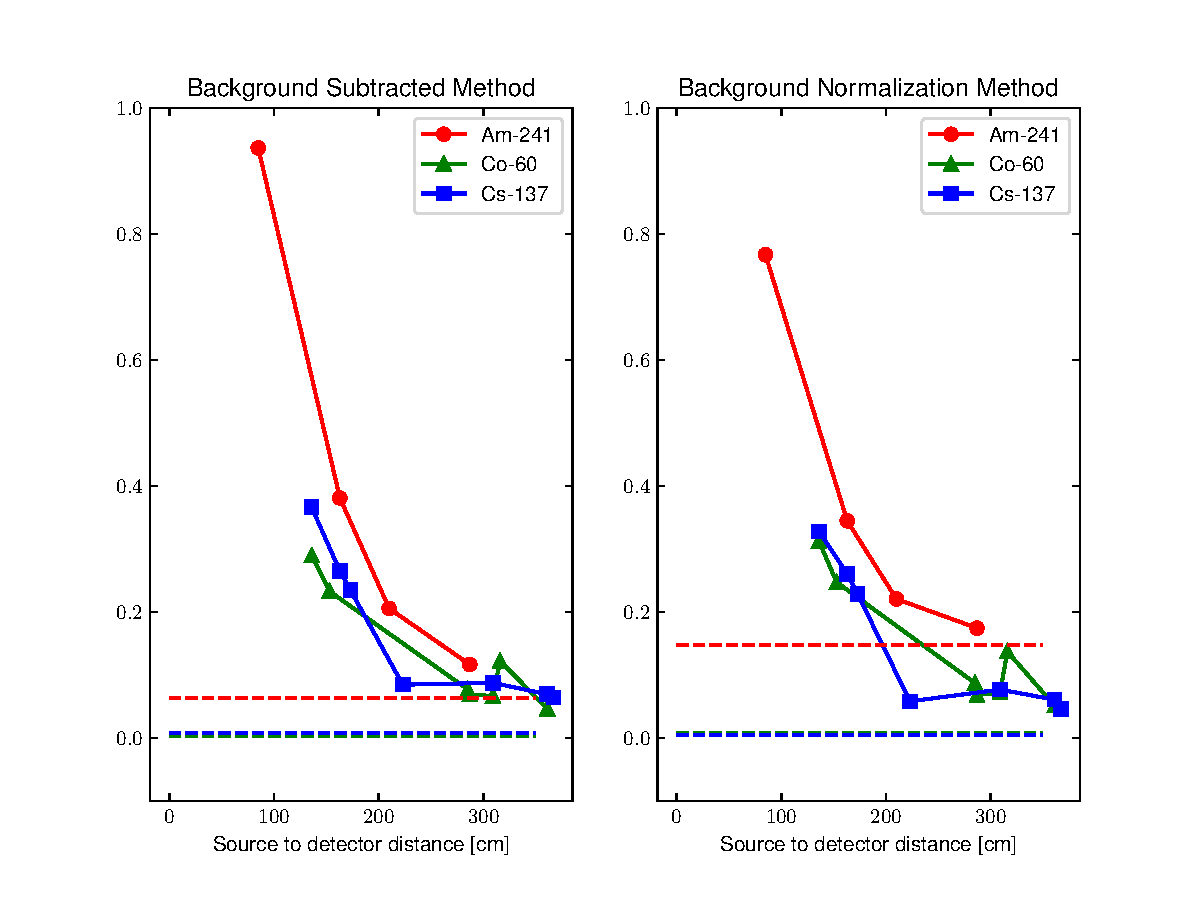
\includegraphics[width=\linewidth]{newfigures/fit_contributions.pdf}
\caption{Variation of estimated radionuclide signal levels as a function of source-to-detector distance.
The coefficients obtained from spectral unfolding represent reference-based relative signal levels rather than absolute activities. The horizontal dashed lines indicate the mean coefficients obtained from measurements in which the corresponding radionuclide was absent, and were used as practical decision thresholds for discrimination. As the distance increases, the estimated coefficient decreases because of geometric attenuation and reduced net detector response. The plotted results are representative data; each condition was repeated more than 10 times under identical settings, and the variation in the overall trend was negligible..}
\label{fig:fi_fitcontrib}
\end{figure}

\end{document}